%!TEX program = xelatex
\documentclass[10pt, compress]{beamer}
\usetheme[titleprogressbar]{m}

\usepackage{booktabs}
\usepackage[scale=2]{ccicons}
\usepackage{minted}
\newcommand\myheading[1]{%
  \par\bigskip
  {\Large\bfseries#1}\par\smallskip}

\usepgfplotslibrary{dateplot}

\usemintedstyle{trac}

\title{Augmented Reality and GIS}
\subtitle{}
\author{Ockert Malan}
\institute{}

\begin{document}

\maketitle

\begin{frame}[fragile]
\frametitle{What is Augmented Reality?}
\myheading{What Wikipedia says:}
\textit{``Augmented Reality (AR) is an interactive experience of a real-world environment whereby the objects that reside in the real-world are 'augmented' by computer-generated perceptual information..."}
\end{frame}

\begin{frame}[fragile]
\frametitle{What is GIS?}
\myheading{What Wikipedia says:}
\textit{``A geographic information system (GIS) is a system designed to capture, store, manipulate, analyze, manage, and present spatial or geographic data."}
\end{frame}

\begin{frame}[fragile]
  \frametitle{Combining AR and GIS}
  Take for example the scene behind this wall...
\begin{figure}
  \centering
 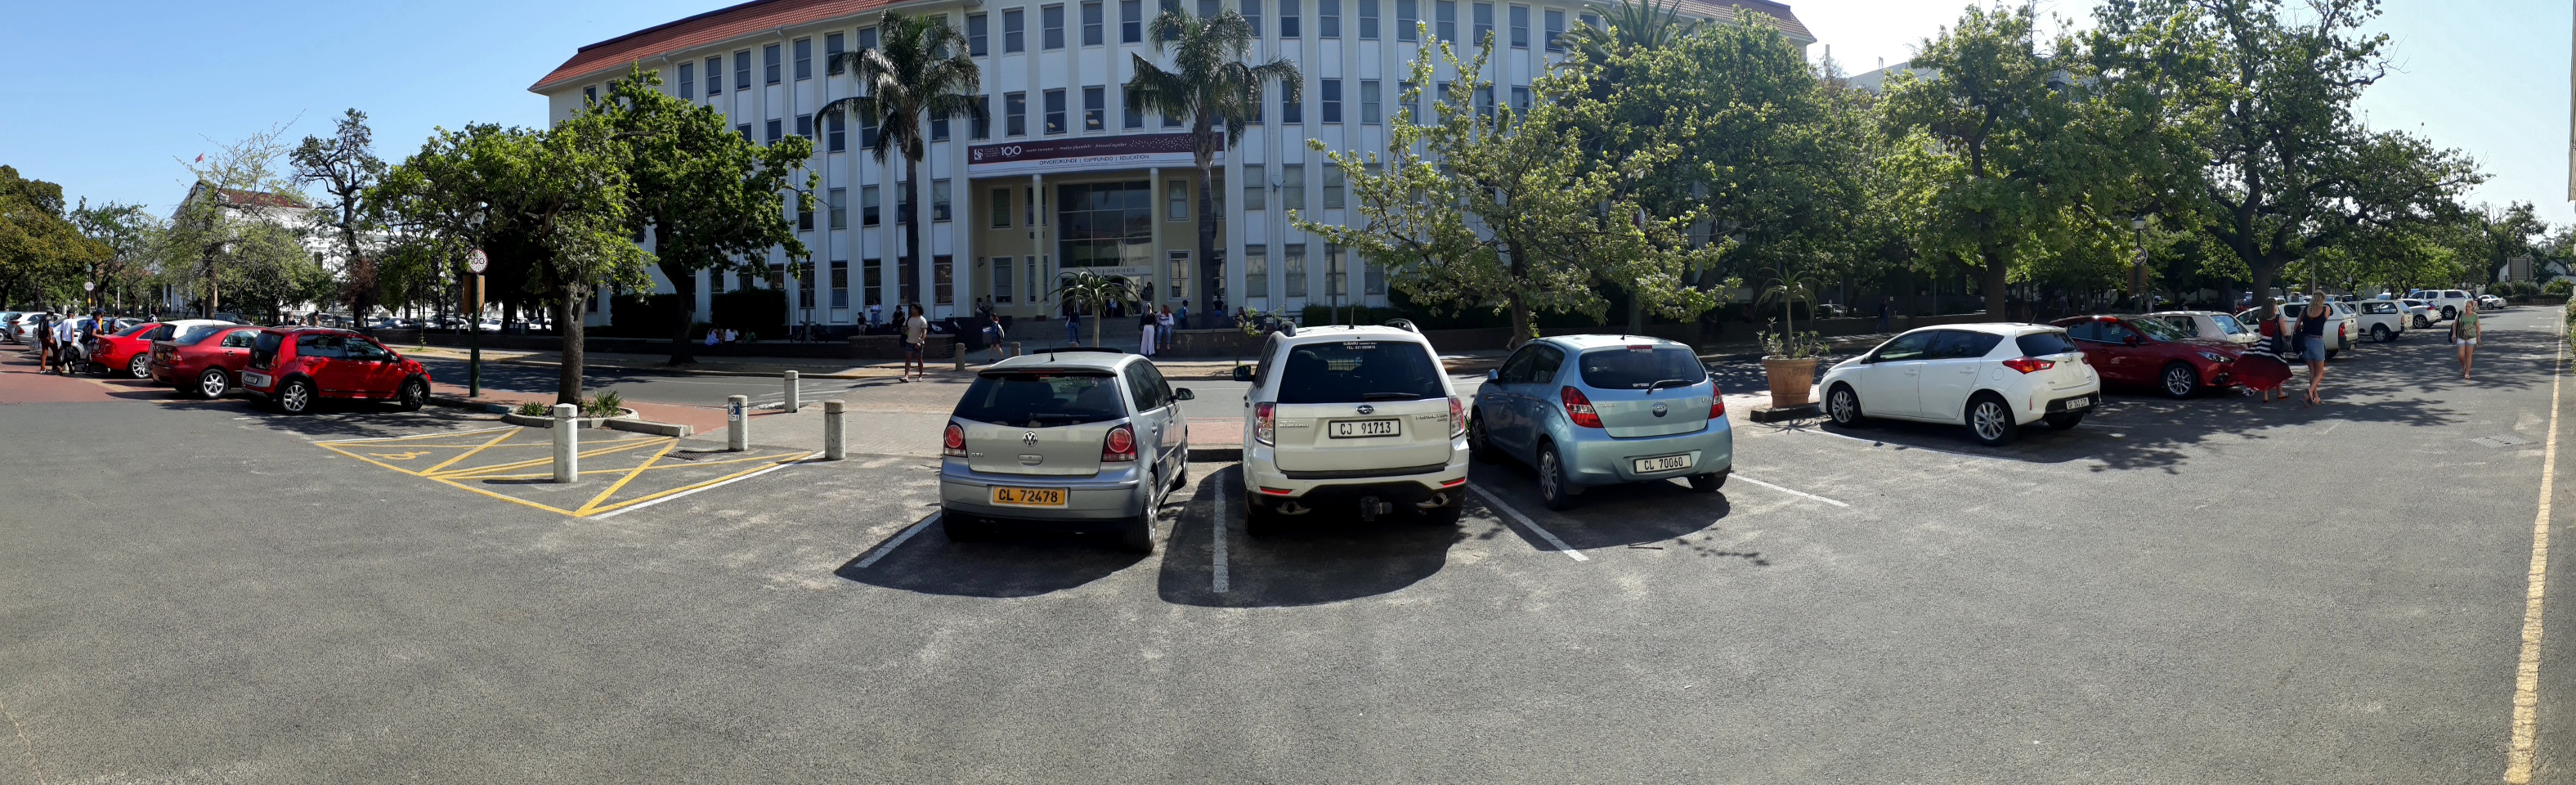
\includegraphics[width=11cm,height=3.5cm]{1.jpg}
\end{figure}
\end{frame}

\begin{frame}[fragile]
  \frametitle{Combining AR and GIS}
  ...as well as the spatial data that can be contained about it in a GIS.
\begin{figure}
  \centering
 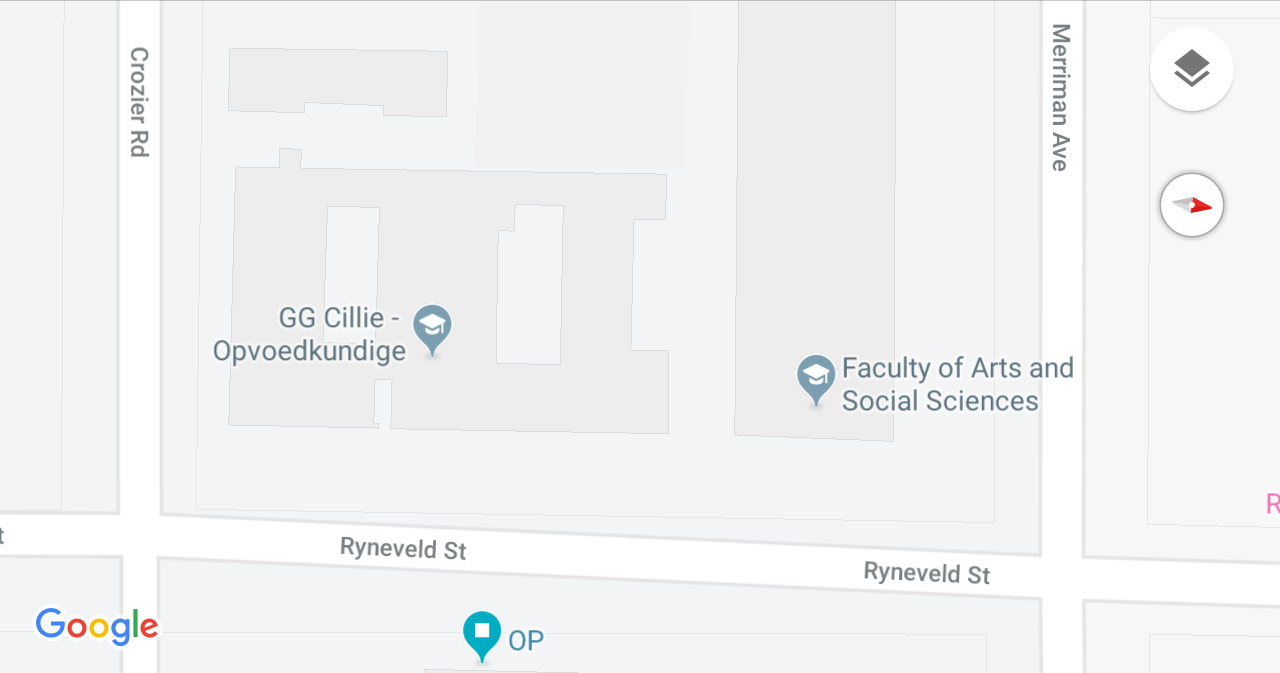
\includegraphics[width=11cm,height=5cm]{2.png}
\end{figure}
\end{frame}

\begin{frame}[fragile]
  \frametitle{Combining AR and GIS}
  This information can then be displayed on the scene itself using AR:
\begin{figure}
  \centering
 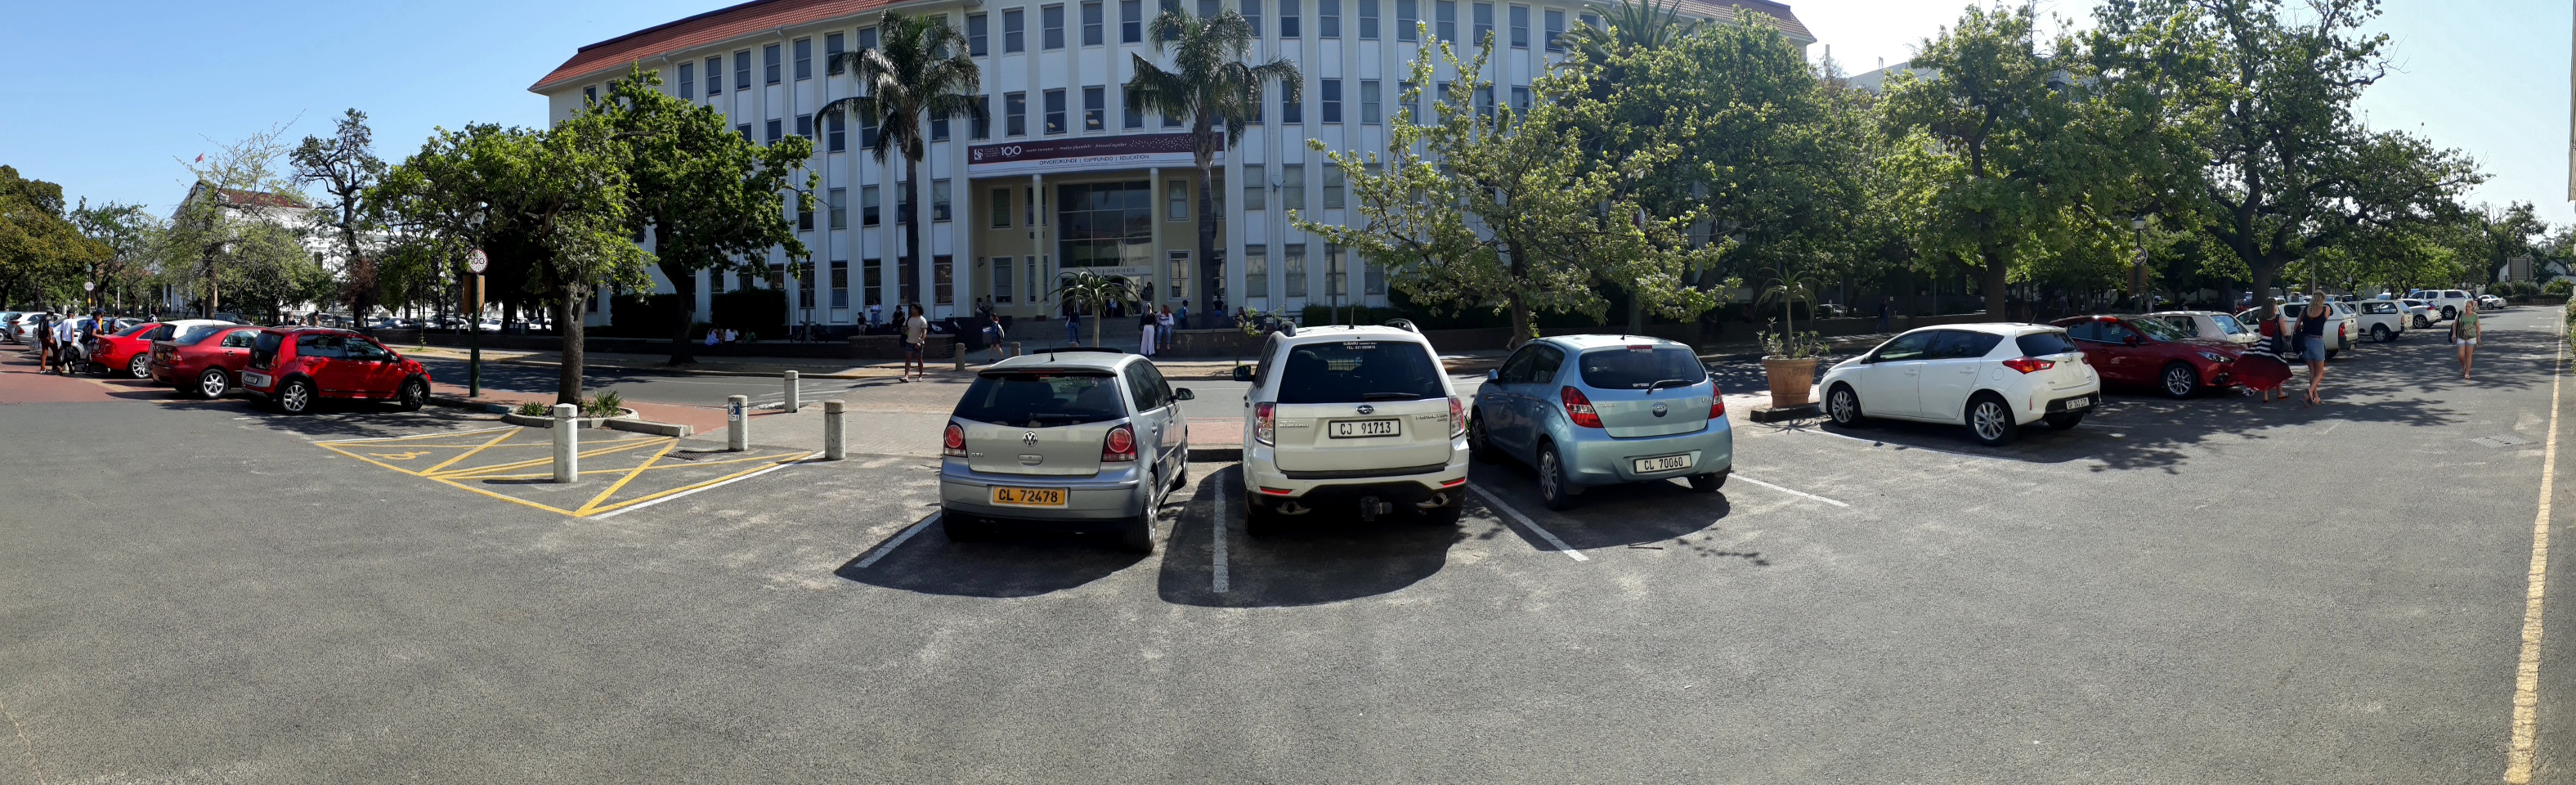
\includegraphics[width=11cm,height=3.5cm]{1.jpg}
\end{figure}
\end{frame}

\end{document}
